%%%%%%%%%%%%%%%%%%%%%%%%%%%%%%%%%%%%%%%%%%%%%%%%%%%%%%%%
%%%%%%%%%%%%%%%%% START 1_ARTICLE.tex %%%%%%%%%%%%%%%%%%
%%%%%%%%%%%%%%%%%%%%%%%%%%%%%%%%%%%%%%%%%%%%%%%%%%%%%%%%
    \begin{adjmulticols}{2}{0mm}{0mm}
\chapter{Background and First Step of the Method}%titlen skal evt. flyttes EFTER \lettrine
\lettrine[lines=2]{\bfseries\color{black}B}{rainstorms generate ideas} and can take many forms. To facilitate an inspiring and free-flowing ‘storm’, our team has a tradition in which, during seminars, we engage in brainstorms while lying comfortably on mattresses. We relax and let our brains work momentarily in a slightly altered state of consciousness, compared to the well-known cognitive state present while in a sitting position. Being a team of researchers who also teach, publish, debate, sing, play, network and collaborate on creating general knowledge about our profession, we gather once a year for a four-day working seminar to allow for time to work in depth. This year, the focus of our mattress brainstorm was to define the theme for an international conference we will host in 2019. 

We understand this state of consciousness in our supine brainstorm as a movement from the so-called primary thinking process into a tertiary thinking process, first defined by the German psychoanalyst Günther Ammon (1974).  Eschen (2002)  brings a simple overview of different modes of thinking as identified by Ammon and Rycroft (1972):%\columnbreak
    \blockquote{Dream-like thinking or (following Freud) ‘primary process thinking… displays  \textit{condensation and displacement}, i.e. images tend to become fused and can readily replace and symbolize one another… ignores the categories of space and time… Secondary process thinking obeys the law of grammar and formal logic… and is governed by the reality principle’. (Eschen 2002, p.17)}
Ammon (1974) further reflects that what is called `real’ is often only what is outside and can be seen by others. This means that dreams and fantasies are identified as `non-real’, even if they are an important reality for the psyche. Thus, he offers the concept of ‘tertiary process thinking’ to describe thinking in creative processes, where one can easily oscillate between primary and secondary process thinking, which involves ego boundaries being more or less open, open to the partner and open to our un- or preconscious, as well as to our emotions. 

In our brainstorming process, while lying down, we let ourselves speak out words and sentences that emerged from the primary thinking process. One  colleague, who was standing up, wrote the words in many different directions and patterns on a whiteboard (see Figure 1).
\FloatBarrier
\noindent
\begin{figure}[H]
\centering % centering kan tilføjes her (optional)
\caption{Brainstorm Notes} % caption indstillinger er under preamble/macros
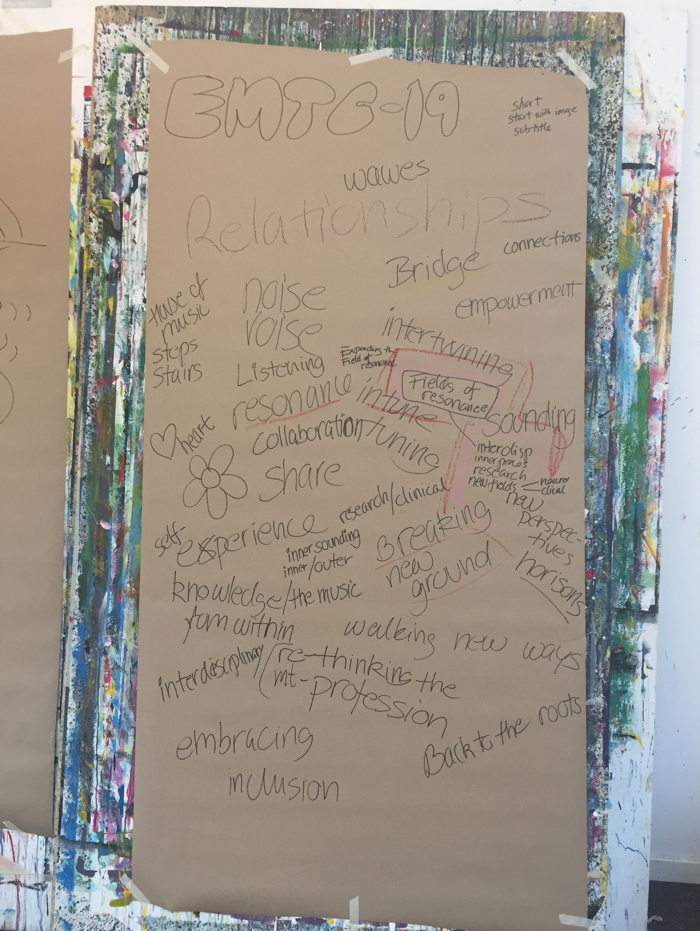
\includegraphics[width=0.9\linewidth]{paper2/p2_data/p2-fig1.png}
\label{fig:p2:1}
\end{figure}
\FloatBarrier
Many considerations, words and concepts came up during the brainstorm, e.g. waves, relationships, bridges, connections, empowerment, sounding, listening, resonance, collaboration, tuning, sharing, embracing, inclusion, new perspectives and horizons. After this procedure, we all moved to a sitting position and started a tertiary thinking process of grouping the words into different themes. During this procedure, it was clear that many of the suggestions were interesting without \textit{being the theme} for our objective, namely to develop a title for a forthcoming conference. When one colleague pronounced the words ‘fields of resonance’, we all resonated immediately with this suggestion, and everyone knew \enquote{this is it}!

We think that a preconception of experiencing, which we define later in this article as psychological resonance, is to allow oneself to be in and operate from both a primary and a tertiary thinking processes, combined with the capacity for empathy, here understood as a concept that implies that one is both:
    \blockquote{…feeling oneself into the object and remaining aware of one´s own identity as another person. (Rycroft 1972, p. 42 as cited in Eschen 2002, p. 18)}
After a further process of cognitive reflection and discussion, we fully agreed on the conference theme: \textit{Fields of Resonance}.%
    \pagenote{European Music Therapy Conference, 2019. See website at \url{www.EMTC19.aau.dk}.}
\par
The next day, we saw an open call from the journal \textit{\theJournal{}} for a special issue on \textit{Resonant Research}! Highly inspired by this coincidence (or synchronicity), we decided to embark on a joint musical and writing project following our joint thinking process of developing the title, in order to reflect together on the concept of resonance. We wanted to improvise in music and to write together in a resonant way by listening to and relating to each other’s contributions. We took turns in the writing process. Since resonance is a complex concept, we expected to learn from this joint exploration and to be prepared on an academic and creative level for the conference. It was also our aim that this internal learning process should be disseminated in a way that could enable others to gain insight from our process and findings. We are used to working with music, improvisation and teaching according to problem-based learning processes, and therefore our team may bring new and different perspectives to resonance processes. 

In the project, resonance is primarily explored from a musical perspective, as all colleagues in this group of ten researchers are involved in music therapy research and university teaching.%
    \pagenote{Aalborg University offers BA, MA and PhD programmes in music therapy, including a 2-year part-time programme in Copenhagen, at the Department of Communication and Psychology.}
We are specifically interested in how we can define the concept of resonance from both an acoustic/physiological and a phenomenological/psychological perspective, and we want to explore these perspectives as intertwined in music therapy practice and in research generally. Therefore, we include a description and an evaluation of the creative and resonant methodology that includes both musical improvisation and resonant writing, which we see as a way of deepening a phenomenological research approach.

\chapter{Method and process: Further Steps}
The submission deadline for the journal left us with a timeframe of about half a year to investigate the concept, collect, analyse and interpret data, and end up with a written academic text. We appointed a ‘guide’ (the first author of this article) to keep an overview of the process, set up a timetable, coordinate and keep us on track regarding the content. We decided on a system of writing in turns, each of us ‘holding the baton’ for a specific time period. The baton consisted of the joint text about resonance, which was shared on an online forum where all colleagues had editing access. During the working process, we did not follow a given method or structure, but when we look back we realize that we intuitively developed or discovered what could be called a nine-step procedure of resonant collaborative writing. The procedure will be described in more detail in the conclusion; the following are only headlines: 1) a creative brainstorm on the phenomenon in focus; 2) exploring the phenomenon and potential conceptual frameworks individually; 3) focusing on the theme/concept/phenomenon in a group discussion of the individual essays; 4) exploring the phenomenon in a musical group improvisation (recorded); 5) processing the improvisation experience individually through arts-based analysis and description techniques; 6) sharing and discussing the individual essays as a basis for a new round of group writing; 7) combining and editing all reflections and text in a more structured and limited draft article; 8) exploring process and preliminary results in a second improvisation (recorded, but only shared verbally immediately afterwards); 9) final editing by a few colleagues. In the following text, some of these steps (2, 4 and 5) are elaborated more than others.

\chapter{Methodology and the Intimacy of Resonant Writing}
In this phenomenological process of writing and musicking \textit{with} resonance \textit{about} resonance, the group members addressed each other as colleagues/peers. This form created a kind of intimacy and internal understanding that is mostly irrelevant for external readers; however, it was important for obtaining insight and for understanding the essence of resonance. The progress of the paper was informed by our internal improvisational logic when developing the theme, and in preparing for publication a more reader-friendly structure was used, with passages separated or merged in order to bring out a more distilled understanding.

The writing process in itself was free and explorative, but it also included insights from creative, musical and metaphorical reflection and investigation. This way of gaining new insight is based on an explorative approach to research, in which researchers investigate processes, interactions and open systems in a flexible way but with a clear requirement to remain systematic, sceptical and ethical (Ridder \& Bonde, 2014; Robson, 2011). The overall research approach was phenomenological, with the aim of describing and understanding the essence of resonance (Jacobsen, Tanggaard \& Brinkmann, 2015). Our understandings and pre-understandings were based on our first joint thinking process during our brainstorm, as well as on the perspectives derived from our social worlds as musicians and therapists, and therefore also our (more or less individual) social constructions. We may be in a position to bring out a perspective on resonance that integrates our music therapy practices. By integrating arts-based methods (Skov, 2013) in an introspective autoethnographic approach (Baarts, 2015), we are able to open up to insights and understandings that allow the phenomenon to emerge. This may help us to set our own academic and explicit pre-understandings and expectations aside (allow the tertiary thinking process to be momentarily active) and meet the unexpected, thus bringing forth new insight. 

\section{Conceptual Dramework for the Understanding of Resonance}
The following section is a summary of step 3 in the process. This is followed by a section describing, analysing and interpreting the first group improvisation (step 4). 

From a musical perspective, we see two major areas of resonance: one of acoustics and physiology, where energy, frequency and vibration come together in observable forms, and one that is a psychological and phenomenological area of lived experiences where forms of emotions come together and are shared, shaped and transformed in the music. The first area consists of observable, even measurable, physical vibrations; the second is of a metaphorical nature, often referring back to the first.

\subsection{Physical Vibrations and Acoustic Resonance}
In our Semester 1 course in music psychology, the students are introduced to the physical area of resonance, often presented using short videos showing beautiful, symmetrical patterns.%
    \pagenote{See, for example, the YouTube clip on resonance at \url{https://www.youtube.com/watch?v=wvJAgrUBF4w}.}
These visible patterns are formed when sand is vibrated by different acoustic sound frequencies, for example by drawing a violin bow across the edge of a brass plate scattered with sand. Matter resonates with sound (sine) waves in an impressive and immediately perceptible way, in a process often called \enquote{cymatics} (Jenny, 2004).  Cymatics is explored by artists, for example using the phenomenon to create audio-visual artworks, and by scientists, for example when deciphering dolphin language or diagnosing heart diseases. In cymatics, energy, frequency, and vibration come together and show visually how sound can shape and order physical matter.%
    \pagenote{Cymatics: see also the website \url{http://www.cymascope.com}.}
\par
A classic experiment used to illustrate resonance is that of two tuning forks (with the same pitch): as the first is played, the other starts to sound \textit{without} being played. This re-sounding or oscillation may also be explicated by the German synonym ‘Mitschwingung’, which may be directly translated as ‘sympathetic vibration’.

\subsection{Psychological and Dyadic Resonance}
Unfortunately, we cannot similarly illustrate or document how the human body and mind resonate with more complex sound patterns of music in as simple or direct a way as in cymatics. The knowledge of sound and music as an ordered and ordering universe, however, has been known since antiquity, when Pythagoras discovered the natural law of tones and overtones (‘harmonics’) and suggested the healing properties of structured sound. The metaphor of ‘good vibrations’ was well established long before the Beach Boys had their global hit in 1966. Therefore, we suggest an analogy between cymatics and music therapy, focusing on the potential of transforming something ‘chaotic’ into clearer and more meaningful patterns as the common denominator. Just as sounding a metal plate can bring random pieces of matter into geometrical shapes, so can music and music therapy be used to facilitate meaningful interactional patterns and relationships between people. Music may facilitate the creation of a resonant relationship with therapeutic possibilities. This power of social cohesion may be illustrated by processes that make thousands of people clap, sing and play%
    \pagenote{See, for example, the 1000 musicians playing for Foo Fighters at \url{https://www.youtube.com/watch?v=JozAmXo2bDE}.}
together in synchrony, but also by smaller groups of people musicking together.

Developmental psychologist Daniel Stern emphasized the impact of resonance on intersubjectivity: ‘I cannot imagine any fundamental base for intersubjectivity without resonance, or sympathy by whatever mechanism’ (Stern 2004, p. 90). This has inspired Danish psychologist and expert in neuroaffective developmental psychology Susan Hart to describe \enquote{dyadic resonance}. According to Hart (2006), dyadic resonance is not achieved through reflection or abstraction, but through affective interaction or reciprocity. Two-way communication and interaction is highly complex, and therefore also difficult to describe, understand and explore, but, by coining the term ‘dyadic resonance’, Hart combines complex neuropsychological, psychodynamic and developmental theories. This explains how humans may synchronize through implicit bodily senses and as such through the autonomous nervous system.

When two persons attune to each other, they do this through multimodal responses. In order to characterize these, we must turn to musical concepts such as pulse, tempo, pitch, melody, harmony, dynamics and form (Ridder, 2017). The responses connected to resonance, and to attunement or empathy in general, are, according to empathy researchers Zaki \& Ochsner (2012), not only related to explicit knowing and mentalizing, but also to prosocial concerns. In order to understand such processes, we may therefore need to expand research in the neuroscience of empathy and add an understanding of ‘neural resonance’ (ibid., p. 675). We see this definition as a further development of this concept from that of Rycroft (see p. 2). In line with dyadic resonance, neural resonance includes deeper and more subtle processes observed in motor intentions, sensory experiences and visceral states (ibid.). 

\subsection{Resonance and Implicit Knowledge in Music Therapy}
In music therapy literature, resonance is often understood as resounding with the different emotions in a musical interaction (Watzlawick, 2004), as sympathetic resonance (a harmonic phenomenon wherein a formerly passive string or vibratory body responds to external vibrations to which it has a harmonic likeness) (Robarts, 2006), as voice resonance (when the client uses his/her voice in order to show more acoustic amplitude) (Haneishi, 2001; Storm, 2013) or as moments of affective resonance with persons suffering from dementia, based on the implicit resonance of the therapist (Coomans, 2016).

In clinical practice, resonance involves subjective and objective interactions through the triad of music, client and therapist. The resonating tones in musical instruments and voices can be seen as metaphors for the process between human beings in the therapeutic space. When the music therapist is attuning to the client, he/she also listens to the silent space between the two. One colleague describes it as follows as of our resonance exploration: 
    \blockquote{I try to use my own body sensation and nervous system as a tuning fork, and to vibrate with/attune to the mood of my client. It can be through communicating with words, with musical sounds in improvisations, or through sharing a music listening experience. I listen to the shared feeling of the moment, and I tune in, trying to create a shared experience.}
In other words, music therapy is close to what resonance is: as a relational process, over time, it includes a starting point, a sounding movement and a subsequent vibrating sounding answer (Lindvang, 2010). This fundamental process is similar to early communication with infants. It is an innate communicative musicality that is present throughout the lifespan in all our creative and communicative expressions with other people (Malloch \& Trevarthen, 2009). 

Tuning in to the resonant field between therapist and client is vital in supporting and guiding the therapeutic process, so that, for example, reactions connected to traumatic experiences can be resolved without overwhelming the client. When the client brings painful material into the therapeutic space, the bodily sensations and feelings of the therapist are set in motion, and the therapist recognizes in a bodily sense what is going on in the client—usually before this is verbalized by the client. This process is called ‘empathic countertransference’ by the late music therapy pioneer Mary Priestley (1994). Hence, the therapist may use resonance to know when to regulate the intensity (up or down) of his/her contact and interactions. Priestley talks of the therapist being aware of the sympathetic resonance of the patient´s feelings through his/her own emotional and/or somatic awareness. She also emphasizes the importance of the therapist’s clarity of thought, in order to articulate these emotions consciously for therapeutic use.  Thus, she introduces an epistemological idea of ‘the transformation from an intuitive sense to information that can be shared’. (Priestley, 1994: p. 87) This understanding is in line with that of psychoanalyst and psychotherapist P. Casement, who claims that 
    \blockquote{Therapists therefore have to develop an openness to, and respect for, feelings and experiences that are quite unlike their own. The greater freedom they  have to resonate to the unfamiliar  ‘keys’ or dissonant ‘harmonies’ of  others , the more it will enhance their receptivity to these unconsciously  interactive cues that are often  central to an understanding of  patients. (Casement, 2014, p. 83)}
From this, it seems clear that music therapy is a treatment that facilitates processes on implicit as well as explicit levels. The therapist engages implicitly and uses his/her knowledge of how to be with other people, and acts explicitly when reflecting and putting into words ‘what’ this means (Hannibal, 2014). This is a unique feature when engaging in musical improvisation where the therapist and the client (and also musicians) play sounds, rhythms, tones, harmonies, melodies, merging them to a musical gestalt where random sounds may become coherent musical statements. Therapist and clients need to listen, be aware and resonate, or to allow the other person to resonate with them. This leads to rapport, intimacy and intersubjectivity. Resonating with one another is a core feature of music therapy at the implicit level, but it may also involve explicit reflection and creation of meaning by negotiating language and creating narratives in the verbal realm. This can be illustrated with the following case vignette from a colleague’s therapeutic work in psychiatry.
    \blockquote{A woman is in the termination phase of long-term psychiatric treatment and is on her way to recovery. There has been a lot of talking, but in this session we start with an improvisation. There is no explicit agenda. Her music is calm and played in three different ways on the piano as she differentiates between the deep, middle and high notes. The therapist creates a musical framework and matches the client’s music. Afterwards, the client says spontaneously: ‘The high notes are all my thoughts, the deep ones are my sadness, and the middle ones are where I have my feet on the ground. I want to explore the middle ones more.'}
This example shows how resonance in music can move from implicit to explicit knowledge, and how musical resonance can deepen a verbal statement and in that sense connect the implicit and explicit levels of relationship and communication. With some client groups, the implicit level is dominant, and with others both the implicit and the explicit resonances act as a facilitator for the therapy. This leads to the concepts of listening attitudes and perspectives for developing sensitivity and an openness to experiencing the emotions that emerge (Pedersen, 1997). The therapist needs to have a disciplined sensitivity and openness, allowing him/herself to move in and out of the resonant field and to translate the experiences into symbolic music or other symbolic languages (Pedersen, 2007a).

\section{Resonant learning}
To summarize the preceding description of resonance, we can say that we cannot separate ourselves from each other or from the world, but, at the same time, separateness is needed to create resonance. Resonance is an oscillation, an interaction between several elements of both intrapsychic and interpsychic nature. This paradox cannot be resolved, but we can deepen our listening skills and our awareness of how we are affected and how we affect our surroundings. We may question whether therapeutic competencies can be learned. In her research on students’ development of therapeutic competencies, Lindvang applied the term ‘resonant learning’ (2010), since these competencies cannot be learned alone. She described how the learning of these competencies was made possible through the music’s ability to create physical as well as psychological and social movement. When teaching groups, resonant learning can be amplified when students are asked to give each other feedback. A mix of cognitive and arts-based feedback (e.g. drawing or poetic writing) is recommended in order to provide a space for resonance.

According to Rosa (2016), the opposite of resonant learning is alienation. This does not imply dissonance, since dissonance is still a way of resonating, although perhaps not experienced in a pleasant (=harmonious) way. When two strings on a violin are played simultaneously and are close to a perfect fifth, but without quite reaching it, the vibrations are experienced more strongly. In this sense, a ‘perfect’ attunement is not necessarily the same as a strong resonance understood as (physical) vibrations. Affect attunement is defined as the parent’s attempt to share an experience of inner state with her child, \textit{without} a wish to change anything (Stern 1985/1991). This may be understood as a state like the ‘perfect fifth’. Stern uses concepts like re-attunement or purposeful misattunement when the parents want to change the inner state of the child, for example wanting to encourage or calm the child (Stern 1985/1991). A healthy developmental environment is not without dissonance; actual development happens when difficulties are solved. Children develop through attunement, misattunement and re-attunement (Hart, 2006; Hart \& Bentzen, 2013). Therefore, therapeutic resonance and resonant learning may gain from dissonance, but not from alienation.  

\chapter{Exploring and Processing the Resonance Phenomenon Through Group Discussion and Musical Improvisation}
The next step in our exploration was a group discussion on our process and how each of us resonated with the themes of the discussion. This discussion identified the need for a joint musical improvisation resonating with the pre-discussion for each colleague. The group improvisation is described below by integrating musical notations, analytic reflections, poetic writings, drawings and graphical notations made by the colleagues individually and here condensed in a way that illustrates the process and the most central reflections.  

\section{Arts-Based Input and Processing}
Before reading the poetic description and graphic notation of the musical improvisation, we recommend that the reader listens to this improvisation on the following link: \url{https://www.youtube.com/watch?v=9Q50bC714yE&t=192s}. 

\noindent First, a poetic description of the improvisation experience:
\par
    \blockquote{A cracking egg\\
    Sensing where\\
    Anybody home?\\
    Vibrating anticipation\\
    Unpredictable harmony\\
    Spontaneous order\\
    Let´s move\\
    We beat the rhythm\\
    Our anguish is a song\\
    Together ahh\\
    Reliving the moment again\\
    There is no doubt\\
    A clear focus of something\\
    Only partly connected\\
    A growing formation of sound\\
    Can we do it?\\
    Will it survive the constant change?\\
    The steady flow of new ideas\\
    I belong\\
    To the rhythm\\
    I am\\
    Us}
\par
\noindent In the ‘worst case’, a group improvisation is pure chaos (everybody makes sound, nobody listens); in the ‘best case’, it is multi-resonant interaction (freedom and spontaneous expression experienced through listening and (re)sounding). The poem above gives one perspective on our musical improvisation, as do the graphical notations in Figures 2 and 3. Graphical notation is a didactic, arts-based method using descriptions and interpretations to create a primarily non-verbal overview and understanding of a musical improvisation (Bergstrøm-Nielsen, 2010); here, the purpose is to identify signs of resonance in the music. The following is a verbal and graphical description and an interpretation made by one colleague:

The 16½--minute improvisation can be described as consisting of two main parts. In the first part, a meeting between initial single sounds led to moments of imitation between the instruments and voices, developing into a shared rhythm in 4/4 time, which accelerated and then faded out.
    \end{adjmulticols}
\FloatBarrier
\noindent
\begin{figure}[htb]
\centering % centering kan tilføjes her (optional)
\caption{Graphical notation of the musical improvisation on resonance, part 1} % caption indstillinger er under preamble/macros
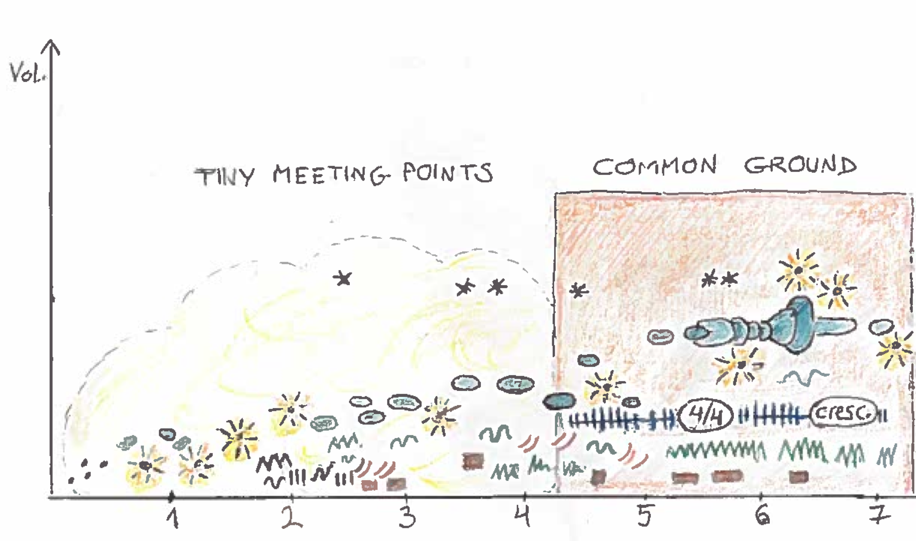
\includegraphics[width=0.9\linewidth]{paper2/p2_data/p2-fig2.png}
\label{fig:p2:2}
\end{figure}
\FloatBarrier
    \begin{adjmulticols}{2}{0mm}{0mm}
The second part started with a period of call-response playing with pauses, and is called ‘negotiation’ in the graphical notation. Then, several voices sang together on the note D, supported by the piano and guitar/bass, and a feeling of sharing on an emotional level emerged. The piano players improvised over an Arabian (Phrygian dominant) scale, still joined with the voices, and the drums started to play a heavy 6/8 rhythm, giving the image of moving along together in a caravan. Maybe the negotiation and emotional sharing was a preparation for the caravan setting out? The improvisation ended with single cracking sounds, some of them metallic. It was as if the group took a break, but there seemed to be more energy, and miles ahead to go.
    \end{adjmulticols}
\FloatBarrier
\noindent
\begin{figure}[htb]
\centering % centering kan tilføjes her (optional)
\caption{Graphical notation of the musical improvisation on resonance, part 2} % caption indstillinger er under preamble/macros
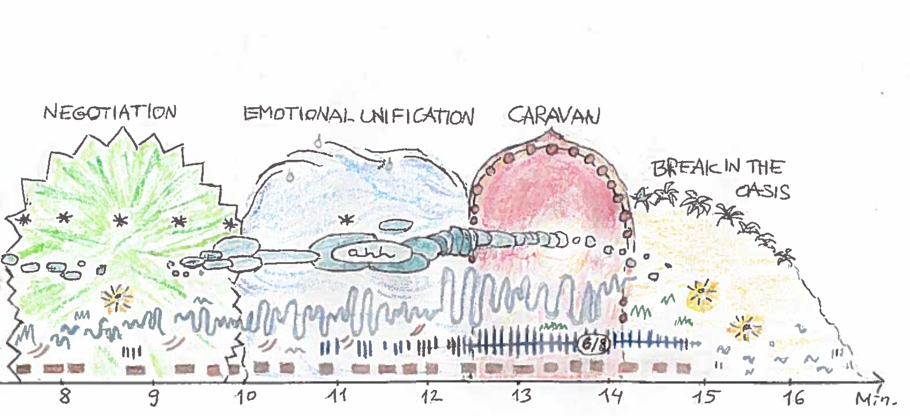
\includegraphics[width=0.9\linewidth]{paper2/p2_data/p2-fig3.png}
\label{fig:p2:3}
\end{figure}
\FloatBarrier
    \begin{adjmulticols}{2}{0mm}{0mm}
\par
Resonance can be sensed and described in the episodes of imitation between instruments (marked with stars in the notation), the two periods with common rhythmic ground, and the period with a strong flow of long vocal notes called ‘emotional unification’.
\noindent
\begin{figure}[H]
\centering % centering kan tilføjes her (optional)
\caption{} % caption indstillinger er under preamble/macros
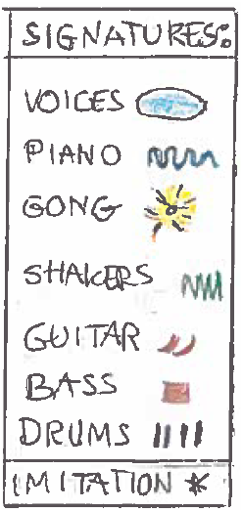
\includegraphics[width=0.5\linewidth]{paper2/p2_data/p2-fig4.png}
\label{fig:p2:4}
\end{figure}
\par
As an addition to the graphical notation, the colleague who made it notes that, while playing, she was not aware of the sense of wholeness of the music, but was focused on playing and listening. When she re-listened to the improvisation and did the analysis, it gave her ‘a feeling of the strength of our group of colleagues, that we are able to find or meet each other on a deeper level, share moments of beauty, and move together with strength’. 

Other colleagues described the improvisation from an internal perspective influenced by the specific instrument they played, but with clear similarities between descriptions. One colleague described the improvisation as follows:
    \blockquote{What will emerge? I feel present and prepared for sensitive listening. Tuning myself into the here and now—leaving thoughts and worries behind me. Striking or banging the gongs—a deep sound flows throughout the room, while ´clicks´ and ´clacks´ and many small sound-forms are moving in and out of my sensation of being part of the total field of sound. Like the gong is the backboard of a sound picture—I feel familiar with chaotic sounds—they make me curious and searching—where are we going—together or apart? Trying out small crashing sounds on the edge of the gongs alternating with flowing banging sounds from the centre of the gongs—sounding together gradually—moving from me to we—in the group sound: following the emerging rhythm and density of the sound—resonating together—everyone being like metaphoric strings and soundboards simultaneously—or are we taking turns?}
Common descriptions of the improvisations among the authors were that it was concentrated, focused and dynamic, and that it evoked feelings of thankfulness and respect.

\section{Emerging Metaphors}
One colleague made a drawing that he called \enquote{Spiralling the Labyrinth}. The title may appear to refer to a chaotic, unpleasant and maybe even anxiety-provoking experience; however, the author describes the opposite: he felt open and safe enough to allow himself to explore an unknown order (the labyrinth) in a free, spontaneous and curious way (spiralling). Spiralling the labyrinth was a nice experience that also brought forth a second metaphor: the \textit{soundboard}. A soundboard is the body of a string instrument such as a piano, guitar or violin, this colleague writes; without this, the strings would have almost no sound. A demonstration of the soundboard effect is to strike a tuning fork and place it on a (wooden) table. This amplification is a special kind of resonance, and in some ways the soundboard is the best metaphor for a music therapist at work (and maybe also for a client playing/expressing herself on an instrument). The therapist not only resonates with what and how something is expressed, but also amplifies it with the special timbre of his/her personal soundboard. The expression may become clearer, more understandable, no matter whether it is dissonant or consonant. The client’s voice is often quiet, soft, weak, broken, hesitant or even ‘out of tune’. The soundboard of the music therapist is therefore needed to make the voice and the message audible in the larger (shared) space and bring it into the pragmatic field of interaction. 

Another colleague also uses the soundboard metaphor and describes the difference between this improvisation and improvisations with clients, which often bring a sense of being fixed in a certain perspective of listening and not being able to flow in resonance. The improvisation with colleagues allowed the therapist to soothe herself—being able and allowed to flow with the resonance. This may well reflect the way of working together as a group of colleagues in a collaborative, exploratory field. She describes herself as a string, while the rest of the colleagues offer a resonating soundboard—she sees herself as part of the soundboard, resonating with the vibrating strings of the others, and sometimes being both the vibrating string and the soundboard simultaneously. This string/soundboard metaphor illustrates group dynamics: simply listening—differently but always sensitively – to ‘oneself listening to the others’. This may be what keeps the group dynamic and the resonance in the group alive, she writes.

\chapter{Discussion and Collaborative Writing}
The final part (‘step nine’) of the text is written by the smaller group of authors who had the ‘licence to cut and edit’ the comprehensive experiential and reflexive material. 

Through a deductive process of conceptualization and an inductive process of introspection and listening, we have explored and described resonance in two distinct ways: one of physical vibration and one of psychological processes. The beautifully structured order of physics is appealing when we need to explain complex processes of implicit knowledge, but uncritically explaining psychological processes in a language of physics is not appropriate; however, the concept of resonance lends us some highly useful metaphors for explaining interaction, relationship and group dynamics. But it also leaves us with terms that need careful consideration and clarification in several discussions raised during the collaborative writing and our group discussions. Most importantly, we discussed physical phenomena such as echoing, mirroring, synchrony, reflection and how they are understood and used metaphorically in communication and therapy, and how we distinguish between analogy and metaphor. 

\section{Analogy and Metaphor}
During the improvisation, the concepts of analogy and metaphor emerged. By improvising musically together, the group aimed to create something related to resonance that could reflect all the different topics that emerged in the discussions. The group created a musical narrative of ideas, feelings and thoughts with the aim of explaining and organizing them in \enquote{metaphorical representations} (Barcelos, 2012). During the improvisation, the participants were highly concentrated, trying to connect with the resonance construct, playing or listening to the moment-by-moment sound landscape. Many musical elements and feelings connected with resonance emerged; however, far from all of them were verbalized or written down during the creation of the article. This means that many resonating feelings and sounds were communicated according to an analogical perspective (Smeijsters, 2012). According to Smeijsters, analogy in music therapy has the function of portraying internal states that occur through time, manifested through music. There is equivalence between the expression of musical forms and the form of inner experiences of the client in music therapy. 

\section{Negative Resonance}
Resonance is described as a process of sympathetic vibration (when the sound of a tuning fork makes another fork sound sympathetically). This raises the question of how we should understand \textit{sympathy} as we, so far, have emphasized the positive and sympathetic aspects of resonance. This notion, however, is not always true. A historical example of resonance as an unwanted physical phenomenon is the collapse of the Tacoma Bridge in 1940. Another example is when a crystal glass splinters as a reaction to a very high soprano note. Resonance as a social phenomenon could in certain situations also be seen as unwanted. Incidents that invoke hatred, fear and xenophobia can cause groups of people to react overheatedly, leading to a negative and rigid discourse or perhaps to violence.

We need to question whether the overuse (or biased use) of the term resonance should be avoided, and at least treated with caution in documenting therapy and research. We have, for example, used resonance as a metaphor for transference and countertransference. We are aware that feelings or moods evoked in oneself in the interaction with another person can never be a ‘true’ insight. A therapist must be highly aware of his/her own inner state before suggesting that an emotion is a reflection of another person’s inner state. As the Danish psychologist Svend Brinkmann states: ‘... mak[ing] decisions by your gut feeling [...] is a bad idea. Especially if you have eaten kale.’ (2014: p. 23 l. 5, our translation). But this should not hinder a professional introspection as long as the subjective impression of the world is treated with caution, curiosity and humility. Resonance between humans is not an either-or (a judgement) but something felt or unfelt (a phenomenological experience).

\section{The Opposite of Resonance}
The German sociologist Hartmut Rosa published a work of 800 pages on resonance (Rosa, 2016) describing human beings’ relation to the world. Rosa argued that \textit{alienation} is the opposite of resonance. Resonance has to do with sensing the body, sensing that expressions make impressions, and experiencing that all that lives is vibrant and in motion. In music therapy, musical communication is used to reduce isolation and alienation to each other, to the world and to ourselves, taking place in the specific time and rhythm that the concrete interaction and situation allows for. But, as Rosa also points out, we cannot instrumentalize resonance: we cannot in any simple way control the field of resonance between humans in the same way as when making, in a controlled manner, a tuning fork oscillate at specific frequencies. In therapy, resonance is a complex phenomenon (Lindvang, 2015).

Coming back to sympathetic vibration, the understanding of resonance is not to be understood as the avoidance of \textit{dissonance}. One colleague writes of how, in the shared group improvisation, she moved in and out of classic harmonies and dissonance. She experienced a change during the improvisation where, although still sounding dissonant by musical standards, she felt more and more resonant in doing so, which vitalized her and led her to move into the more harmonic field with ease and without feeling a pressure of resonance as harmony and harmonies. Resonating in dissonance can be very transformative.

\section{Subtle Nuances} 
This leads to an overall understanding of group dynamics and of how these may be directed in a way that allows for dissonance but without leading to overheating. Group dynamics can become evident or be experienced differently when playing or improvising music together. One author describes how, during the improvisation, she became conscious of how she knew some colleagues better than others, and was drawn to some types of music more than to others, which was related to her expectations and her familiarity with the group as a whole. In this way, there might be a difference between knowledge of each other, feeling connected and feeling in resonance with each other.

The subtle nuances between knowing, connecting and resonating are important to define. Professor Tony Wigram offered a range of improvisational terms and techniques in his book on clinical improvisation (2004) that may be helpful in defining such differences. As an example, he differentiated between mirroring, imitating or copying on the one hand, and matching on the other. He described matching as a technique where ‘the therapist’s music is not identical to the client’s, but is the same in style and quality’ (p. 84). Finally, he described empathic improvisation and reflecting that allows for two separate musical identities, but asks for a musical interpretation or empathic confirmation (p. 89). Empathic reflection is a powerful way to match the emotional content of the other; it is more than harmonics and percussive sounds, and we suggest that we must understand musical matching differently than emotional matching. Stern (2010) argued that Wigram´s (2004) concept of matching in music therapy can be characterized as affect attunement and that it ‘is at the base of so much of the relationship and the transmission and communication between therapist and child’. He also described it as a vital technique in emotional communication: ‘Music is fabulous at [affect attunement]’ (ibid, p. 94), and he believed this type of intersubjective contact to be the single most necessary aspect of any successful therapy, because it is a type of contact that two people can expand on.

\section{Resonant Exploring}
The following section is a summary of the group’s reflections on the process and the method.  The experience of our group improvisation fostered new reflections about resonance. Complexity emerged, and it became clear that resonance in music therapy is a multilayered phenomenon, since it happens on several levels of our being. Various theoretical ways of understanding were also mentioned. It is interesting for music therapy that resonance is a dynamic concept that can be understood from more than one theoretical perspective. Through this exercise, where we investigated the concept of resonance and reflected on the lived experience of resonance, a genuine integrative understanding of ourselves and of our profession of music therapy seems to have emerged. 

Furthermore, our different experiences of the improvisation revealed different perspectives on the phenomenon of resonance. When members of a group try to empathically resonate with each other, it is not possible to predict what will be perceived by the individual participant. This seems to require maintaining humility in trying to understand each other. There is a need to trust one's own senses and feelings in a disciplined way, since human compassion is the most vibrant instrument to bring into our exploration of relationships. At the same time, there is a need to include former experiences and knowledge in order to use introspection as a soundboard for what is expressed and communicated. For new knowledge to occur, subjectivity needs to be ‘disciplined’, which calls for self-experiential training, either as a researcher or as a professional therapist, as well as ethical thinking. In qualitative research, as well as in therapeutic processes where subjective phenomena or inner states are explored, specific competencies are required of the researcher/therapist: first of all, the ability to listen deeply without being absorbed by either the sound or the emotional experience of the other or by one’s own sound or emotional experience or idea of what is going on. Working with the multilayered phenomenon of resonance demands training of the consciousness to let go without losing ground and to take part without taking over.

\section{Reflections on Methods in Collaborative Writing and Publishing: A Nine-Step Model}
Writing with resonance means writing in a way that facilitates the connection between the writer(s) and the reader. In the first phases of the present inquiry, we were writing about resonance in a process where we were connecting with each other: we shared our experiential knowledge, our personal repertoire of cognitive, emotional and embodied experience (Meier \& Wegener, 2016). A significant change occurred in the working process when we turned introspection to ‘outro-spection’, letting the group step out of a heuristic incubation and into explication and creative synthesis. The process of editing is a transformation of a text to something that can be shared with a broader public. A reciprocal group resonance must be transferred to resonance with potential readers. Since resonance is a process that is dependent on the engagement and experiences of two parts, it is our hope that the reader reaches what Wikan describes as ‘the commonality of experience’ (Wikan, 2012, in Meier \& Wegener, 2016). In other words, we might see this project as an exercise in searching for both internal and external resonance.

Usually, a manuscript for a journal is presented as the final product of many work phases, in an established format often involving many discussions and dialogues between the authors (and editors), which are intangible to the reader. In the present case, the dialoguing process has been transformed into a product and becomes accessible to other people. We do hope that our paper can be used as a demonstration of how collaborative resonant writing can be used to collectively discuss and explore a theme. We assume that it is not unusual in a team of educators and researchers for a number of phenomena to be central/pivotal, although still difficult to grasp and describe. Even well-known concepts may be understood differently. 

We do not see this article as a final product, but as an illustration of a work in progress that has opened our minds to a hilly landscape and the possibility of developing new fields of resonance and more clarity – over time.

\section{The Discovery of a Resonant, Collaborative Procedure}
In order to learn from each other, we applied a phenomenological and introspective approach to research, and intuitively we developed or discovered a nine-step procedure for resonant collaborative writing (emerging as we moved along):
\begin{enumerate}
    \item A creative brainstorm on the phenomenon in focus: as a preparation for the brainstorm, we lay down and entered a slightly altered state of consciousness, allowing ourselves to express words from a primary and later tertiary thinking process to reach a joint agreed theme for the conference.
    \item Exploring the phenomenon and potential conceptual frameworks individually: in the first round, we wrote our initial thoughts about the concept of resonance, its overall relevance to our profession (music therapy) and how we have experienced resonance in practice.
    \item Focusing on the theme/concept/phenomenon in a group discussion of the individual essays: after this first round, we met. We summarized and discussed the process and shared the experiences and reflections we had had in the resonant writing project so far. This was immediately followed by:
    \item Exploring the phenomenon in a musical group improvisation (recorded): after our talk, we went to a music room equipped with a large variety of musical instruments and did a free improvisation. Our focus for the improvisation was embedded in the previous talk, and we were allowed to do whatever we liked, to listen and/or play in order to investigate resonance from both an individual and a shared perspective. The recorded improvisation was shared.
    \item Processing the improvisation experience individually through arts-based analysis and description techniques: the improvisation, lasting 16½ minutes, was shared on our online forum.%
    \pagenote{The sound file of the improvisation is available by following this link: ------.}
    The improvisation experience was then processed in a new round, in whatever way each of the ten researchers found natural: by notation, analytic reflections, poetic writings, drawings or graphical notation.
    \item Sharing and discussing the individual essays as a basis for a new group writing round: our reflections, thoughts, questions and new insights on the phenomenon were put into words by passing the baton and by reflecting on the input from the group. Highly interesting metaphors emerged in the process.
    \item Editing all reflections and text together in a more structured and limited draft article: the text was structured, shortened and edited, mainly by the guide, but with responses and suggestions from the group. Redundant passages were deleted, language reviewed and the text divided into thematic sections with draft headings. The aim was to create fluency and clarity while retaining the multiple layers and flow of information with the many movements back and forth.
    \item Exploring process and preliminary results in a second improvisation (recorded, but only shared verbally immediately afterwards): the team gathered again, and the inquiry was rounded off with one more improvisation – this time only with voices and in an old church with impressive acoustics. The 15-minute improvisation allowed the group once again to experience musical resonance and to find inspiration as to ways of summarizing, concluding and reflecting on perspectives.
    \item Final editing by a few colleagues: the whole process had up to this point in time been focused on our own wish to learn about and explore the concept of resonance. Our internal writings were therefore transferred to a text relevant to readers outside our group interested in the concept and in our method. After deciding in the group how to structure a final article, a small group of colleagues were given the licence to cut and edit.
This procedure may be possible for other groups to follow—the steps that imply musical improvisation can be performed with other arts-based/creative methods.
    \end{enumerate}

\chapter{Conclusion and Perspectives}
The main finding of the collaborative exploration can be formulated as follows: resonance is a visible and ordered phenomenon consisting of physical vibrations and acoustic sounding that offers a clear logic. Furthermore, it is used metaphorically to describe and understand complex psychological processes of human relationships. Each of the rounds in the nine-step procedure contributed in a unique way to an embodied understanding of the phenomenon. The concluding discussions of the writing process included one more focused but free improvisation in our group (step 7). The team was gathered for our summer seminar at the old monastery in Ørslev. After a long day with hours of professional discussions, we went to the old church of the monastery in the gentle evening light. We felt the silence and the calm atmosphere embracing us as we stood in a circle ready to improvise together with our voices (link to the improvisation). After this improvisation, the group gathered in the evocative living room at the monastery. In a circle, each of us shared their personal experience of the improvisation, as well as reflections on the collaborative research process. One colleague had a spontaneous comment about the improvisation: 
    \blockquote{It was like a feeling of giving. I enjoyed that. I had an experience of being strengthened. We were resonant, we were listening, following. We could move around. In a coherent way.}
One person in the group expressed the improvisation as a kind of release:
    \blockquote{In the writing process, I experienced some feelings of insecurity. I was not sure that I had something to add. There are so many possibilities around this theme. So I had some difficulties finding my voice in collaborative writing. In the improvisation, I found a soft voice and I felt that we all met. Being vulnerable and insecure was okay. Later, I raised my voice more.}
Several in the group described a feeling of accomplishment and safety during the improvisation, and several used the metaphor of being together in a common playground. It is interesting how creative interactions like improvisations in sound can open up to a redeeming and uplifting mood, and at the same time make room for various feelings and bring new perspectives on serious themes to explore. Finally, the group said that they felt highly inspired by resonating verbally and in music. This led to a playful atmosphere with a series of several clear and concrete (and also some crazy) ideas for how to organize a conference entitled \enquote{Fields of Resonance}.
    \end{adjmulticols}